\section{Appendix to Section 4 -- Auxiliary Concepts to Operational Semantics}
\label{app:aux}

Lemma \ref{lemma:orig:to:bounded}  states that
 any execution  which is part of an execution which started at some initial state, is scoped by that state.
 
  \begin{lemma}
\label{lemma:orig:to:bounded}
For all $\overline M$, all $n,m\in \mathbb{N}$ with $m\leq n$, $\sigma_0$, ... $\sigma_n$,  $\sigma_{init}$, $\sigma$, $\sigma'$, where
$\sigma_{init}$ is an initial state:
 \label{otbTwo}
\[\leadstoOrigStar {\Mtwo} {\sigma_{init}}  {\sigma}\ \wedge\ \leadstoOrigStar {\Mtwo} {\sigma}  {\sigma'}\ \ \Longrightarrow\ \  \leadstoBoundedStarThree {\Mtwo} {\sigma} {\sigma_{init}} {\sigma'}\].
 \end{lemma}
 \begin{tabular}{lll}
\begin{minipage}{.5\textwidth}
Revisit  Fig. \ref{fig:UpSemantics} (copied here), and assume that $\sigma_6$ is an initial state where
an initial state's heap contains a single object of class \prg{Object}, and
its  stack   consists of a single frame, whose local variable map is a mapping from \prg{this} to the single object, and whose continuation is  any statement. 
%(See Definition %s \ref{def:initial} and  \ref{def:arising} and the {appendices %of the full paper \cite{necessityFull}}.
\end{minipage}
& \ \  \   &
\begin{minipage}{.45\textwidth}
\begin{tabular}{|c|}
 \hline %  \\ -- this added one vertical space
\resizebox{6cm}{!}{
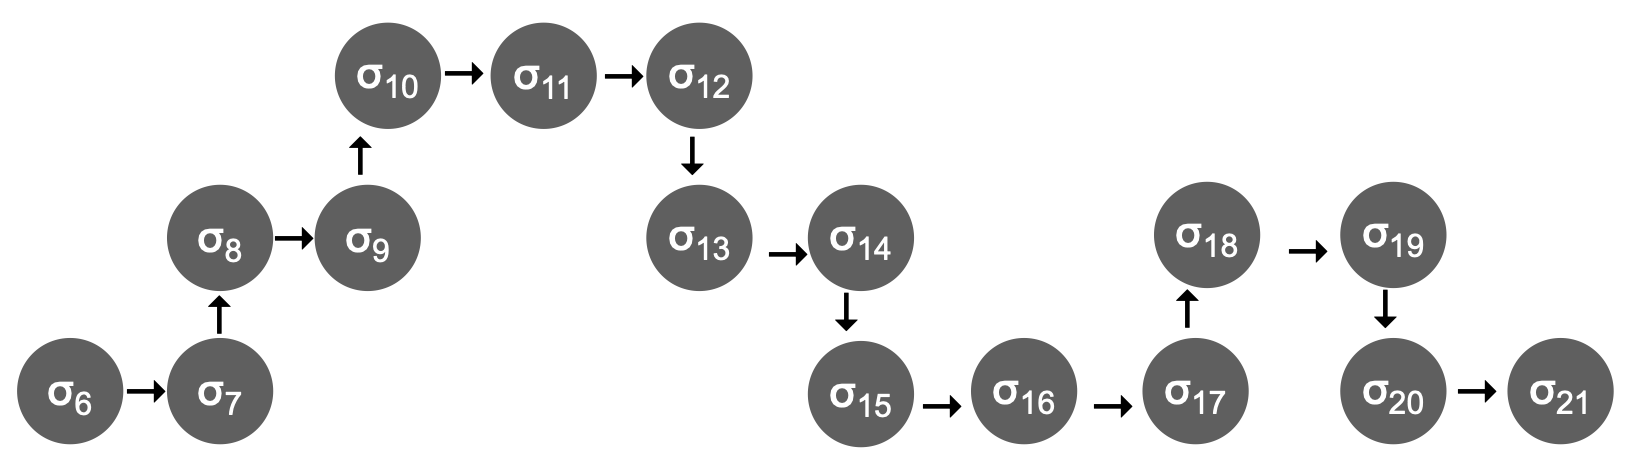
\includegraphics[width=\linewidth]{diagrams/bounded2.png}
} 
 \\
\hline

\end{tabular}

\end{minipage}
\end{tabular}
We have  $\leadstoOrigStar {\Mtwo} {\sigma_{10}}  {\sigma_{14}}$ and $ \notLeadstoBoundedStar {\Mtwo}  {\sigma_{10}} {\sigma_{14}}$.
However, because $\sigma_6$ is an initial state, we have $\leadstoBoundedStarThree {\Mtwo}  {\sigma_{10}} {\sigma_{6}}  {\sigma_{14}}$ -- \cf Lemma \ref{lemma:orig:to:bounded}.

%%%%%%%%%%%%%%%%%
Lemma \ref{lemma:call:return}
states that method calls  correspond  to pushing of frames (here $\sigma_2 \in \PushS  {\interpret {\sigma_1} {y}} {\sigma_1}$),
 that they leave the values of the caller's local variables unmodified ($\forall z. \interpret {\sigma_1} {z} = \interpret {\sigma_4} {z}$), and
method returns  correspond  to popping  a frame  (here $\sigma_3 \in  \PushSLong  {( {\interpret {\sigma_1} {y}},{\overline \alpha})} {\sigma_4}$), where the local map of the frame being popped contains the original arguments ($\overline {{\interpret {\sigma_1} {y}}}$) as well as some additional addresses ($\overline \alpha$).
The latter property -- that  the frame being popped from $\sigma_3$ contained the original arguments passed in to $\sigma_2$ -- holds because 
 we forbid assignments to formal parameters (but we do allow  assignments to the other local variables).
 
 
 \begin{lemma}
 \label{lemma:call:return}
 For any modules $\Mtwo$, states $\sigma_1$, $\sigma_2$, $\sigma_3$, and $\sigma_4$, variables $x$, $y_0... y_n$:
 
 $  
   \left. %\{
   \begin{array}{l}  \ \strut \ \ \sigma_1.\prg{cont}\txteq x:= y_0.m(y_1,...y_n);\_ ,\\
    \ \strut \ \  \leadstoOrig {\Mtwo} {\sigma_1}   {\sigma_2} , \\
     \ \strut \ \  \leadstoBoundedStarFin  {\Mtwo}  {\sigma_2}  {\sigma_3}, \\
  \ \strut \ \  \leadstoOrig {\Mtwo} {\sigma_3}   {\sigma_4}, 
    \end{array} 
\right \}
 \mbox{implies} \ \ 
  \begin{cases}
     \ \strut \ \  \sigma_2 \in \PushS  {\interpret {\sigma_1} {y}} {\sigma_1},\\
     \ \strut \  \exists z.\ \sigma_3.\prg{cont}{\txtin z} \\
       \ \strut \ \       \forall z. \interpret {\sigma_1} {z} = \interpret {\sigma_4} {z},\\  
        \ \strut \ \       \exists \overline \alpha. [\ \sigma_3 \in  \PushSLong  {( {\interpret {\sigma_1} {y}},{\overline \alpha})} {\sigma_4} \ ]
    \end{cases} 
$
 \end{lemma}
 
 \sdN{
 \beginProof{lemma:relevant}
Take a  module sets $\Mtwo$, states $\sigma$, $\sigma'$,   addresses $\alpha$, and $\overline \alpha$, variables, $x$, $\overline {y}$,:

\begin{enumerate}
\item

Assume that $ \sigma'\!\in\! \PushS {\alpha} {\sigma}   \ \wedge  \  {\overline \alpha} \subseteq \LRelevantO  {\sigma}$, and
 that $\alpha \in \LRelevantO {\sigma'} $

TODO

Therefore, $\alpha \in \LRelevantO   {\sigma}$
\item
This is proven by induction on the length of the derivation. We consider one step:

Assume that ${\leadstoBounded  {\Mtwo}  {\sigma_1} {\sigma}    {\sigma_2}}$, and that $\alpha \in dom(\sigma) \cap \LRelevantO {\sigma_2}$.

TODO

Therefore $\alpha \in  \LRelevantO {\sigma}$
\end{enumerate}

\completeProof
}
